\appendix

\section{Log of pre-specified experiments}\label{app:prereg}
Each row is an experiment script (\texttt{experiments/expNN\_*.py}) with the short hash of the commit that first added it, before it was run, and the date. The first line of each script's docstring is quoted. Scripts were revised after a first run only where stated in their docstrings (experiments 47, 49, 57; each revision is a separate commit and the first version is retrievable). Experiments 1--16 belong to the earlier theory paper on sequential certificates and are not used here.
\begingroup\scriptsize\setlength{\tabcolsep}{3pt}
\begin{longtable}{@{}rllp{9.8cm}@{}}
\toprule
\# & Commit & Date & Purpose\\
\midrule
\endhead
17 & \texttt{98de084} & 2026-10-23 & Experiment 17: scaling with graph size and ablation of CERT-CD.\\
18 & \texttt{0318781} & 2026-10-23 & Experiment 18: held-out simulated pair families, sample-size sweep, baselines.\\
19 & \texttt{0318781} & 2026-10-23 & Experiment 19: sensitivity of the Tuebingen result to the random seed.\\
20 & \texttt{c5cd9b0} & 2026-10-23 & Experiment 20: real physical data with a known causal graph (Causal Chambers).\\
21 & \texttt{269ae7a} & 2026-10-23 & Experiment 21: direction of the known edges of the Causal Chambers.\\
22 & \texttt{aa99d05} & 2026-10-23 & Experiment 22: nonparametric sequential adjacency certificate vs the linear primitive.\\
23 & \texttt{aa99d05} & 2026-10-23 & Experiment 23: nonparametric adjacency certificate on the Causal Chambers.\\
24 & \texttt{9f32aaa} & 2026-10-23 & Experiment 24: Causal Chambers with conditioning-set order k = 3.\\
25 & \texttt{7045b1b} & 2026-10-23 & Experiment 25: the nonparametric certificate on the exp13 and exp17 DAG data.\\
26 & \texttt{b59a1c6} & 2026-10-23 & Experiment 26: PC with the same nonparametric test, under monitoring.\\
27 & \texttt{ba2f7ac} & 2026-10-23 & Experiment 27: untouched Causal Chamber recordings, final algorithm frozen.\\
28 & \texttt{06bffaf} & 2026-10-23 & Experiment 28: abstaining comparison of the pair rules at matched coverage.\\
29 & \texttt{f85302f} & 2026-10-23 & Experiment 29: BTAD against PC, GES, DirectLiNGAM and PC with an iid nonparametric test\\
30 & \texttt{ced1b11} & 2026-10-23 & Experiment 30: BTAD on the untouched Causal Chamber recordings, time-ordered.\\
31 & \texttt{9dddc37} & 2026-10-24 & Fit the LRG classifier on exp31 features; choose the threshold on validation; report held-out simulation metrics.\\
31 & \texttt{d682048} & 2026-10-24 & Experiment 31: train the learned replicated-gain skeleton model (LRG) on simulated data.\\
32 & \texttt{9dddc37} & 2026-10-24 & Experiment 32: the frozen LRG model on the untouched, time-ordered Causal Chamber recordings.\\
33 & \texttt{b91cbf1} & 2026-10-24 & Experiment 33: frozen LRG and BTAD on the two Causal Chamber recordings with i.i.d. random actuators.\\
34 & \texttt{985335e} & 2026-10-24 & Experiment 34: train the learned pair-direction model (PDM) on simulated pairs.\\
34 & \texttt{ddb1d8f} & 2026-10-24 & Fit the pair-direction classifier on exp34 features; report held-out simulated accuracy.\\
35 & \texttt{ddb1d8f} & 2026-10-24 & Experiment 35: the frozen pair-direction model (PDM) on real and held-out pair sets.\\
36 & \texttt{5e7f00b} & 2026-10-24 & Experiment 36: Sachs data and NOTEARS, added to the graph benchmark.\\
37 & \texttt{a83a699} & 2026-10-24 & Experiment 37: PC with the nonparametric test on the two i.i.d. chamber recordings (exp20 subsamples).\\
38 & \texttt{c8e01d1} & 2026-10-24 & Experiment 38: LOCI and ANM added to the pair benchmark, and the Sachs pairs.\\
39 & \texttt{6387fdc} & 2026-10-24 & Experiment 39: DAGMA and PCMCI+ added to the graph benchmark.\\
40 & \texttt{ba11744} & 2026-10-24 & Experiment 40: LOCI on the Tuebingen pairs with up to 2000 rows per pair.\\
41 & \texttt{c94369a} & 2026-10-24 & Experiment 41 (negative result): block-ICP pilot on five wind-tunnel walk recordings (development only).\\
42 & \texttt{bbdeb3a} & 2026-10-24 & Experiment 42: 2025-2026 pair rules on the same pair sets as exp38.\\
43 & \texttt{bbdeb3a} & 2026-10-24 & Experiment 43: BF-BIC with BOSS (arXiv 2510.04276) on the graph benchmark.\\
44 & \texttt{cdf776c} & 2026-10-24 & Experiment 44: SNOE-style edge orientation (arXiv 2506.05590, see sprint\_cd/snoe\_lite.py).\\
45 & \texttt{37f8d52} & 2026-10-25 & Experiment 45: published methods with public code on the graph benchmark.\\
46 & \texttt{101841b} & 2026-10-25 & Experiment 46: published pair rules with public code (AVICI pretrained, RESIT) on the exp38 pair sets.\\
47 & \texttt{b805f02} & 2026-10-25 & Experiment 47 (revision 4: the discordance rate and McNemar counts exclude missing values and exact ties, the Bonferroni\\
48 & \texttt{211fb35} & 2026-10-25 & Experiment 48: resolution of the Sachs graph benchmark.\\
49 & \texttt{02dfe48} & 2026-10-25 & Experiment 49: why do direction rules that exploit dependence lose to RECI/IGCI on real pairs?\\
50 & \texttt{c17d1ad} & 2026-10-25 & Experiment 50: does heteroscedastic noise cause the loss of the noise-model rules? (simulation, dose-response)\\
51 & \texttt{31dadda} & 2026-10-25 & Experiment 51: an assumption-gated direction rule (GATE), frozen on simulation, tested once on real pairs.\\
52 & \texttt{4282166} & 2026-10-25 & Experiment 52: controls for experiments 49-50 (leakage-free marginal classifier, matched dose-response with marginal con\\
53 & \texttt{37fc958} & 2026-10-25 & Experiment 53: three further real pair collections from the Causal Chambers, and the diagnostics of exp49.\\
54 & \texttt{37d6d13} & 2026-10-25 & Experiment 54: sorted-conditional compression with the quantisation convention that reproduces its published figure.\\
55 & \texttt{8f63bb7} & 2026-10-25 & Experiment 55: reference implementations from the cdt package, and LOCI/ANM-GP/PDM on the three new collections.\\
56 & \texttt{04de9ce} & 2026-10-25 & Experiment 56: a factorial simulation of the regimes found in exp49-52, with label-free diagnostics.\\
57 & \texttt{241d7b0} & 2026-10-25 & Experiment 57 (revision 3: the observed decisions of the three new collections are the raw-array ones of exp59 (IGCI, RE\\
58 & \texttt{5c1c168} & 2026-10-25 & Experiment 58: pair rules on every untouched Causal Chambers recording (not only the first of each type).\\
59 & \texttt{8b388ce} & 2026-10-25 & Experiment 59: tie handling as a free parameter, and raw-array versions for the three new collections.\\
60 & \texttt{b592bf7} & 2026-10-25 & Experiment 60: TRA on raw arrays for the all-recordings walk pairs (exp58) and the three new collections (exp53).\\
61 & \texttt{d68bf71} & 2026-10-25 & Experiment 61: how much does the evaluation protocol move each rule on Tuebingen?\\
\bottomrule
\end{longtable}
\endgroup

\section{Implementation details}\label{app:impl}
\paragraph{Preprocessing.} T\"ubingen: at most $2000$ rows drawn with a seed that depends on the pair identifier; each variable with tied values dequantised by adding uniform noise in $\pm\frac12$ of the smallest positive gap between distinct values (experiment 14). Chamber and Sachs collections: raw values (Sachs on the log scale with a floor at $10^{-3}$), at most $2000$ random rows; walk recordings use random rows of the first $4000$ rows for pairs and the first $4000$ (graphs) or $2000$ (45) rows in time order for graphs. All rules see the raw arrays; a copy with a $10^{-6}$ range jitter on tied values is used only in the sensitivity analysis of Section~\ref{sec:ties} and in the simulations.
\paragraph{Scores.} All rules return a signed score, positive for $x\to y$. IGCI, RECI, ANM-HSIC and pairwise LiNGAM return a direction label and a magnitude that we convert to a sign. A score of exactly zero counts as half correct (this affected $23$ pairs of the Gaussian-process ANM). A rule that returns no value on a pair (TRA's spline failure) is excluded from that pair and the denominator is reduced.
\paragraph{Compression.} Section~\ref{sec:audit}. In both variants the score is $s=\mathrm{sc}(q_y,q_x)/\max(\mathrm{dc}(q_x),1)-\mathrm{sc}(q_x,q_y)/\max(\mathrm{dc}(q_y),1)$ with $\mathrm{sc}(\mathrm{key},\mathrm{val})=|\mathrm{bz2}(\Delta\,\mathrm{val}[\mathrm{argsort}(\mathrm{key})])|$ and $\mathrm{dc}(q)=|\mathrm{bz2}(\Delta q)|$, a stable sort, differences cast to \texttt{int8}, bzip2 level 9; $s>0$ means $x\to y$.
\paragraph{TRA.} Cross-fitted smoothing-spline residuals ($5$ folds), a rank-uniform point cloud, the total length of the zero-dimensional persistence (minimum spanning tree) in the window $\alpha=\kappa n^{-2/3}$, $\beta=c_\beta\alpha$ with $\kappa=1$, $c_\beta=4$, at most $1000$ rows; the direction is the sign of the difference of the two residual functionals. The conservative variant TRA-C ($B=100$ Gaussian-copula bootstrap draws) took $27$\,s per pair at $n=800$ and was not run.
\paragraph{AVICI.} The pretrained model \texttt{scm-v0}; edge probability matrix of the standardised data ($\le 2000$ rows for graphs, $\le 1000$ for pairs); graphs: skeleton from probability $\ge 0.5$; pairs: $P(x\to y)-P(y\to x)$. Run in a virtual environment with \texttt{jax 0.4.30}, \texttt{flax 0.8.5}, \texttt{dm-haiku 0.0.12}, \texttt{optax 0.2.2}, \texttt{numpy<2}.
\paragraph{Graph packages.} GOLEM (gCastle, $10^4$ iterations), NOTEARS-MLP and GraN-DAG and DAG-GNN (gCastle defaults), GRaSP and BOSS (\texttt{causal-learn}, BIC), RESIT (random forest depth $4$, $\alpha=0.01$) and CAM-UV ($\alpha=0.01$, three explanatory values; \texttt{lingam}); a run over $900$\,s is a timeout.
\paragraph{Marginal-only classifier.} Features as in Section~\ref{sec:marg}; scikit-learn \texttt{LogisticRegression} with $C=1$ on standardised features; both orientations of every training pair; $50$ repetitions of five-fold cross-validation for the first protocol, deterministic splits for the others.
\paragraph{Heteroscedasticity.} Cubic B-splines with six knots on the standardised cause, ridge penalty one, two-fold cross-fitting, residual scale correlation $|\rho_S(|r|,x)|$.
\paragraph{Factorial simulation.} Seeds are \texttt{default\_rng([20263200, mechanism, cause, scale, measurement, n, k])}; the scale of the noise is normalised so that the mean noise variance is $(0.3\,\mathrm{sd}\,f(c))^2$; measurement noise is Gaussian with $0.3$ times the sample sd of each variable.
\paragraph{Software.} Python 3.11, \texttt{numpy 1.26}, \texttt{scipy 1.13}, \texttt{scikit-learn 1.9}, \texttt{statsmodels 0.15}, \texttt{causal-learn 0.1.4.8}, \texttt{lingam 1.13}, \texttt{gcastle}, \texttt{causalchamber 0.2.8}; four CPU cores, no GPU.

\section{Negative results of the algorithm search}\label{app:negative}
Each attempt was fixed before its run. Numbers are strict skeleton $F_1$ or forced accuracy against the reference.
\begingroup\small\setlength{\tabcolsep}{3pt}
\begin{longtable}{@{}p{3.2cm}p{4.3cm}p{7.2cm}@{}}
\toprule
Attempt & Idea & Outcome on real data\\
\midrule
\endhead
CERT-CD (sequential certificates) & assert edges only by rejecting; anytime-valid & False-edge control holds in simulation ($2.7\%$ against $27$--$91\%$), not on the chambers\\
BTAD & block-replicated additive gains & highest precision ($0.60$) but recall $0.16$; $F_1$ $0.25$--$0.28$ on walk recordings\\
LRG & gradient boosting on block-gain features, trained on simulations & $F_1$ $0.36$ (chambers), $0.67$ (Sachs); within-recording AUC $0.55$\\
PDM & pair classifier trained on $40000$ simulated pairs & $95\%$ on simulated pairs, $40.2\%$ on T\"ubingen\\
Block-ICP & invariant causal prediction with time blocks & empty graphs, $F_1\le 0.07$ on development recordings\\
Compression, TRA, BF-BIC (exp 42--43, 54) & re-implemented 2025--2026 methods & compression: $60.8$--$64.7\%$ with the floor256 variant, $66.7\%$ ($74.7\%$ weighted) round255, $38.3\%$ on i.i.d.\ chambers; TRA $64.6\%$ ($86.2\%$ on i.i.d.\ chambers); BF-BIC with BOSS: Sachs $0.67$, walks $0.42$\\
Interventional route (pilot) & shift of each sensor under each intervened actuator (light tunnel) & KS: precision $1.00$, recall $0.72$ ($28$ of $39$ arcs), AUC $0.91$; the missed arcs show no shift; conditional version recall $0.79$ at precision $0.51$\\
Published packages (exp 45--46) & AVICI, GOLEM, NOTEARS-MLP, GraN-DAG, DAG-GNN, GRaSP, BOSS, RESIT, CAM-UV & best: BOSS $0.55$ i.i.d.\ chambers; GRaSP $0.68$, BOSS $0.65$ large-ESS; Sachs $\le0.56$; walks $\le0.37$; many neural timeouts\\
GATE (exp 51) & ANM-HSIC when a symmetric heteroscedasticity diagnostic is low, else RECI & T\"ubingen $65.7\%$ against $60.8\%$ ($p=0.30$); chambers $75.5\%$, $77.0\%$ against $97.9\%$, $94.3\%$\\
Predictive validation (exp 57) & nearest simulated neighbours predict each rule's accuracy & Spearman $0.006$ in the reported revision (needed $0.5$); RMSE $0.31$ against $0.24$ for the constant; real pairs are $2$--$13$ sd from the simulation\\
\bottomrule
\end{longtable}
\endgroup

\section{Additional tables}\label{app:tables}

\begin{table}[ht]
\caption{Accuracy with $95\%$ cluster-bootstrap intervals for every rule and collection (clusters: pairs for T\"ubingen and Sachs, edges for the i.i.d.\ chambers and the three new collections, recordings for the walks); for collections with $8$ or fewer clusters (the five-recording walks, Bernoulli, changepoints, Malus) only the accuracy is given because the interval is degenerate.}
\label{tab:collections_ci}
\scriptsize\setlength{\tabcolsep}{2pt}
\begin{tabular}{@{}lcccc@{}}
\toprule
Rule & T\"ubingen & iid & walks & walks (19)\\
\midrule
IGCI & 0.56 [0.46,0.66] & 0.94 [0.85,1.00] & 0.89 & 0.96 [0.91,0.99]\\
RECI & 0.61 [0.51,0.70] & 0.98 [0.94,1.00] & 0.94 & 0.83 [0.79,0.87]\\
ANM-HSIC & 0.61 [0.51,0.71] & 0.72 [0.61,0.83] & 0.63 & 0.43 [0.38,0.50]\\
Pairwise LiNGAM & 0.61 [0.51,0.70] & 0.78 [0.68,0.87] & 0.71 & 0.67 [0.62,0.72]\\
PDM & 0.40 [0.30,0.50] & 0.93 [0.84,0.99] & 0.84 & --\\
LOCI & 0.65 [0.56,0.74] & 0.77 [0.66,0.86] & 0.68 & --\\
ANM, Gaussian process & 0.55 [0.46,0.65] & 0.77 [0.68,0.87] & 0.67 & --\\
Compression, floor256 & 0.61 [0.52,0.70] & 0.30 [0.19,0.40] & 0.61 & --\\
Compression, round255 & 0.67 [0.58,0.75] & 0.38 [0.29,0.48] & 0.52 & 0.50 [0.43,0.57]\\
TRA & 0.65 [0.54,0.75] & 0.86 [0.77,0.94] & 0.61 & 0.56 [0.50,0.61]\\
AVICI & 0.59 [0.49,0.69] & 0.90 [0.82,0.97] & 0.56 & 0.63 [0.58,0.68]\\
RESIT & 0.61 [0.52,0.70] & 0.71 [0.61,0.81] & 0.65 & 0.48 [0.43,0.53]\\
\bottomrule
\end{tabular}
\medskip

\begin{tabular}{@{}lcccc@{}}
\toprule
Rule & Sachs & Bernoulli & Changepoints & Malus\\
\midrule
IGCI & 0.65 [0.41,0.88] & 1.00 & 1.00 & 0.08\\
RECI & 0.53 [0.29,0.76] & 0.25 & 1.00 & 0.56\\
ANM-HSIC & 0.59 [0.35,0.82] & 0.31 & 0.57 & 0.31\\
Pairwise LiNGAM & 0.53 [0.29,0.76] & 0.88 & 0.43 & 0.40\\
PDM & -- & -- & -- & --\\
LOCI & 0.47 [0.24,0.71] & 0.56 & 0.80 & 0.38\\
ANM, Gaussian process & 0.56 [0.32,0.79] & 0.47 & 0.54 & 0.33\\
Compression, floor256 & 0.76 [0.53,0.94] & -- & -- & --\\
Compression, round255 & 0.65 [0.41,0.88] & 0.50 & 1.00 & 0.60\\
TRA & 0.59 [0.35,0.82] & 0.62 & -- & 0.54\\
AVICI & 0.53 [0.29,0.76] & 0.62 & 0.40 & 0.02\\
RESIT & 0.47 [0.29,0.65] & 0.25 & 0.53 & 0.50\\
\bottomrule
\end{tabular}
\end{table}

\begin{table}[ht]
\caption{The ten reporting universes with at least $30$ pairs per rule: weighting, minimum number of rows, coverage (\%), pairs in the subset, smallest number of pairs evaluated for any rule, and the accuracy of each rule (a subset of the columns of Table~\ref{tab:multi}; CmpF: round255 compression; the other four columns are in the repository file \texttt{results/exp47\_multiverse.json}).}
\label{tab:universes}
\tiny\setlength{\tabcolsep}{1.5pt}
\begin{tabular}{@{}lrrrrccccccccc@{}}
\toprule
Weights & Rows & Cov. & $n$ & min & IGCI & RECI & ANM-H & LiNGAM & LOCI & TRA & CmpF & AVICI & RESIT\\
\midrule
official & 0 & 100 & 102 & 82 & 0.66 & 0.71 & 0.61 & 0.62 & 0.64 & 0.65 & 0.75 & 0.61 & 0.62\\
official & 0 & 75 & 102 & 62 & 0.64 & 0.77 & 0.58 & 0.65 & 0.67 & 0.71 & 0.78 & 0.60 & 0.57\\
official & 0 & 50 & 102 & 41 & 0.66 & 0.87 & 0.57 & 0.74 & 0.63 & 0.74 & 0.88 & 0.58 & 0.47\\
official & 250 & 100 & 76 & 56 & 0.71 & 0.75 & 0.65 & 0.54 & 0.71 & 0.70 & 0.75 & 0.59 & 0.63\\
official & 250 & 75 & 76 & 42 & 0.69 & 0.84 & 0.63 & 0.56 & 0.77 & 0.74 & 0.77 & 0.60 & 0.56\\
none & 0 & 100 & 102 & 82 & 0.56 & 0.61 & 0.61 & 0.61 & 0.65 & 0.65 & 0.67 & 0.59 & 0.61\\
none & 0 & 75 & 102 & 62 & 0.50 & 0.68 & 0.57 & 0.63 & 0.63 & 0.71 & 0.72 & 0.63 & 0.58\\
none & 0 & 50 & 102 & 41 & 0.47 & 0.76 & 0.57 & 0.71 & 0.63 & 0.76 & 0.84 & 0.65 & 0.55\\
none & 250 & 100 & 76 & 56 & 0.55 & 0.67 & 0.70 & 0.55 & 0.72 & 0.68 & 0.71 & 0.54 & 0.66\\
none & 250 & 75 & 76 & 42 & 0.51 & 0.75 & 0.67 & 0.58 & 0.75 & 0.76 & 0.77 & 0.61 & 0.63\\
\bottomrule
\end{tabular}
\end{table}

\begin{table}[ht]
\caption{Sachs: skeleton $F_1$ of $22$ configurations with a $95\%$ bootstrap interval over the $55$ variable pairs.}
\label{tab:sachs_ci}
\small
\begin{tabular}{@{}lcc@{}}
\toprule
Configuration & $F_1$ & interval\\
\midrule
LRG & 0.67 & [0.42, 0.85]\\
BF-BIC+BOSS & 0.67 & [0.42, 0.85]\\
PC-GCM $\alpha=$0.01 & 0.64 & [0.38, 0.83]\\
PC-GCM $\alpha=$0.05 & 0.62 & [0.36, 0.81]\\
BTAD & 0.62 & [0.35, 0.81]\\
PC $\alpha=$0.05 & 0.58 & [0.30, 0.80]\\
GES-BIC & 0.58 & [0.30, 0.80]\\
AVICI & 0.56 & [0.29, 0.77]\\
NOTEARS-MLP & 0.56 & [0.29, 0.77]\\
PC $\alpha=$0.01 & 0.52 & [0.24, 0.74]\\
DirectLiNGAM & 0.52 & [0.24, 0.74]\\
PCMCI+ & 0.52 & [0.24, 0.74]\\
GRaSP & 0.52 & [0.24, 0.74]\\
BOSS & 0.52 & [0.24, 0.74]\\
CERT-CD nonparametric k=3 & 0.45 & [0.15, 0.69]\\
DAGMA & 0.45 & [0.15, 0.69]\\
RESIT & 0.45 & [0.24, 0.63]\\
NOTEARS & 0.30 & [0.00, 0.56]\\
GOLEM & 0.30 & [0.00, 0.56]\\
DAG-GNN & 0.30 & [0.00, 0.56]\\
GraN-DAG & 0.11 & [0.00, 0.32]\\
CAM-UV & 0.11 & [0.00, 0.33]\\
\bottomrule
\end{tabular}
\end{table}

The accuracy of each of the $144$ cells of the factorial simulation is in \texttt{results/exp56\_factorial.json}.


\begin{table}[ht]
\caption{Kendall rank correlation between the orderings of the rules on two collections, with a permutation $p$-value (5000 permutations of one ordering) in parentheses; rules run on both collections, at least five.}
\label{tab:kendall}
\scriptsize\setlength{\tabcolsep}{2pt}
\begin{tabular}{@{}lcccccccc@{}}
\toprule
 & T\"ub. & iid & walks & walks19 & Sachs & Bern. & Chgpt. & Malus\\
\midrule
T\"ubingen & -- & -0.38 (0.11) & -0.30 (0.21) & -0.42 (0.20) & -0.12 (0.68) & -0.19 (0.54) & +0.24 (0.46) & +0.51 (0.06)\\
iid & -0.38 (0.11) & -- & +0.53 (0.02) & +0.57 (0.06) & -0.17 (0.53) & +0.34 (0.21) & -0.03 (1.00) & -0.16 (0.60)\\
walks & -0.30 (0.21) & +0.53 (0.02) & -- & +0.43 (0.18) & -0.27 (0.30) & +0.07 (0.86) & +0.26 (0.41) & -0.02 (1.00)\\
walks19 & -0.42 (0.20) & +0.57 (0.06) & +0.43 (0.18) & -- & +0.04 (1.00) & +0.52 (0.11) & +0.21 (0.65) & -0.07 (0.90)\\
Sachs & -0.12 (0.68) & -0.17 (0.53) & -0.27 (0.30) & +0.04 (1.00) & -- & +0.27 (0.35) & +0.41 (0.18) & -0.02 (1.00)\\
Bernoulli & -0.19 (0.54) & +0.34 (0.21) & +0.07 (0.86) & +0.52 (0.11) & +0.27 (0.35) & -- & -0.06 (0.92) & -0.25 (0.37)\\
Changepoints & +0.24 (0.46) & -0.03 (1.00) & +0.26 (0.41) & +0.21 (0.65) & +0.41 (0.18) & -0.06 (0.92) & -- & +0.26 (0.40)\\
Malus & +0.51 (0.06) & -0.16 (0.60) & -0.02 (1.00) & -0.07 (0.90) & -0.02 (1.00) & -0.25 (0.37) & +0.26 (0.40) & --\\
\bottomrule
\end{tabular}
\end{table}

\begin{table}[ht]
\caption{All $18$ conventions of the compression rule on the $102$ T\"ubingen pairs (quantiser $\times$ row cap; rows thinned linearly above the cap). The published value is $68$ pairs, $74.7\%$ weighted. Source: \texttt{results/exp54\_audit\_conventions.json}.}
\label{tab:grid18}
\small
\begin{tabular}{@{}lcccc@{}}
\toprule
Quantiser & Row cap & Pairs correct & Unweighted & Weighted\\
\midrule
floor256 & 500 & 64 & 0.627 & 0.627\\
floor256 & 1000 & 67 & 0.657 & 0.697\\
floor256 & 2000 & 63 & 0.618 & 0.648\\
floor256 & 4000 & 69 & 0.676 & 0.708\\
floor256 & 8000 & 67 & 0.657 & 0.688\\
floor256 & none & 67 & 0.657 & 0.688\\
floor255 & 500 & 69 & 0.676 & 0.697\\
floor255 & 1000 & 69 & 0.676 & 0.695\\
floor255 & 2000 & 67 & 0.657 & 0.682\\
floor255 & 4000 & 71 & 0.696 & 0.702\\
floor255 & 8000 & 71 & 0.696 & 0.705\\
floor255 & none & 71 & 0.696 & 0.705\\
round255 & 500 & 71 & 0.696 & 0.717\\
round255 & 1000 & 70 & 0.686 & 0.740\\
round255 & 2000 & 69 & 0.676 & 0.744\\
round255 & 4000 & 68 & 0.667 & 0.740\\
round255 & 8000 & 68 & 0.667 & 0.747\\
round255 & none & 69 & 0.676 & 0.753\\
\bottomrule
\end{tabular}
\end{table}

\section{Further mechanism evidence}\label{app:mech}
\subsection{A factorial map}\label{sec:factorial}
To see the regimes together we crossed five factors (experiment 56): the mechanism ($\tanh 2c$, $c^3/3$, $\sin 1.5c$), the cause marginal (uniform, normal, bimodal, five-level discrete), the noise scale (homoscedastic, cause-dependent, independent random), measurement noise on both variables ($0$ or $0.3$ sd), and $n\in\{200,1000\}$: $144$ cells of $25$ pairs ($3600$ pairs), seven rules. Table~\ref{tab:factorial} gives the accuracy by factor level and Table~\ref{tab:factorial2} the interaction of the noise scale with measurement noise.

\begin{table}[t]
\caption{Factorial simulation (3600 pairs): accuracy of seven rules averaged over the other factors.}
\label{tab:factorial}
\small
\setlength{\tabcolsep}{3pt}
\begin{tabular}{@{}llccccccc@{}}
\toprule
Factor & Level & IGCI & RECI & ANM-HSIC & LiNGAM & Compr. & RESIT & AVICI\\
\midrule
mechanism & tanh & 0.66 & 0.71 & 0.42 & 0.16 & 0.65 & 0.46 & 0.66\\
mechanism & cubic & 0.87 & 1.00 & 0.70 & 0.54 & 0.75 & 0.75 & 0.19\\
mechanism & sin & 0.55 & 0.95 & 0.73 & 0.81 & 0.74 & 0.75 & 0.85\\
cause marginal & uniform & 0.94 & 0.95 & 0.52 & 0.34 & 0.84 & 0.53 & 0.49\\
cause marginal & normal & 0.61 & 0.72 & 0.64 & 0.36 & 0.84 & 0.68 & 0.89\\
cause marginal & bimodal & 0.75 & 0.89 & 0.63 & 0.59 & 0.79 & 0.68 & 0.36\\
cause marginal & discrete5 & 0.47 & 0.97 & 0.68 & 0.71 & 0.39 & 0.72 & 0.53\\
noise scale & homoscedastic & 0.56 & 0.82 & 0.82 & 0.50 & 0.68 & 0.84 & 0.55\\
noise scale & cause & 0.74 & 0.90 & 0.28 & 0.56 & 0.72 & 0.36 & 0.66\\
noise scale & independent scale & 0.78 & 0.94 & 0.75 & 0.45 & 0.74 & 0.76 & 0.49\\
measurement noise & 0 & 0.61 & 0.92 & 0.64 & 0.50 & 0.70 & 0.67 & 0.58\\
measurement noise & 1 & 0.77 & 0.85 & 0.59 & 0.50 & 0.73 & 0.64 & 0.56\\
n & 200 & 0.66 & 0.87 & 0.61 & 0.52 & 0.62 & 0.66 & 0.58\\
n & 1000 & 0.73 & 0.90 & 0.62 & 0.48 & 0.81 & 0.65 & 0.55\\
\bottomrule
\end{tabular}
\end{table}

\begin{table}[t]
\caption{Factorial simulation: noise scale $\times$ measurement noise.}
\label{tab:factorial2}
\small
\setlength{\tabcolsep}{3pt}
\begin{tabular}{@{}llccccccc@{}}
\toprule
Noise scale & Meas. noise & IGCI & RECI & ANM-HSIC & LiNGAM & Compr. & RESIT & AVICI\\
\midrule
homoscedastic & no & 0.47 & 0.89 & 0.95 & 0.49 & 0.67 & 0.95 & 0.54\\
homoscedastic & yes & 0.64 & 0.76 & 0.69 & 0.50 & 0.69 & 0.74 & 0.55\\
cause-dependent & no & 0.68 & 0.91 & 0.06 & 0.55 & 0.71 & 0.17 & 0.68\\
cause-dependent & yes & 0.81 & 0.89 & 0.49 & 0.56 & 0.73 & 0.54 & 0.65\\
independent scale & no & 0.69 & 0.98 & 0.91 & 0.46 & 0.70 & 0.89 & 0.52\\
independent scale & yes & 0.86 & 0.90 & 0.60 & 0.45 & 0.78 & 0.64 & 0.47\\
\bottomrule
\end{tabular}
\end{table}

The additive-noise rules are near-perfect only without cause-dependent scale and without measurement noise (ANM-HSIC $0.95$ and RESIT $0.95$ with homoscedastic noise, $0.91$ and $0.89$ with the independent scale), fall to $0.69$ and $0.74$ with measurement noise alone, and to $0.06$ and $0.17$ with a cause-dependent scale; measurement noise partly masks the reversal ($0.49$, $0.54$). IGCI and the round255 compression are the weakest rules when the cause is discrete ($0.47$ and $0.39$; the simulated arrays carry the $10^{-6}$ jitter under which IGCI reverses, Section~\ref{sec:ties}, so the IGCI figure is partly a tie artefact); IGCI is more accurate with measurement noise than without ($0.77$ against $0.61$); the round255 compression depends on $n$ ($0.62$ at $200$, $0.81$ at $1000$); AVICI fails on the cubic mechanism ($0.19$) and is at $0.49$ for the uniform cause. RECI has the highest average accuracy in $12$ of the $14$ factor levels (the exceptions are the normal cause, where AVICI is at $0.89$ against $0.72$, and homoscedastic noise, where RESIT is at $0.84$ against $0.82$). Which factor breaks which rule is rule-specific.

\subsection{An assumption-gated rule fails}\label{sec:gate}
If the regimes explain the T\"ubingen average, a rule that identifies the regime should beat both of its branches. We froze GATE on simulation before touching a real pair (experiment 51): $h_{\min}=\min(h(x\to y),h(y\to x))$, symmetric in the variables, threshold at the $95$th percentile of $h_{\min}$ on $200$ homoscedastic simulated pairs ($0.058$ at $n=500$); GATE returns the ANM-HSIC direction when $h_{\min}\le 0.058$ and the RECI direction otherwise. The pre-specified predictions were an accuracy of at least $0.70$ on T\"ubingen and, on the chambers, within $0.05$ of RECI. Both failed. On T\"ubingen GATE has $65.7\%$ ($77.1\%$ with the official weights) against $60.8\%$ ($70.9\%$) for RECI; it routes $34\%$ of the pairs to ANM-HSIC and the difference to RECI is not significant (exact McNemar $10$ against $5$, $p=0.30$). On the i.i.d.\ chambers GATE has $75.5\%$ against $97.9\%$ ($0$ against $21$ discordant pairs, $p<10^{-6}$) and on the walks $77.0\%$ against $94.3\%$ ($p<10^{-6}$), because it sends $88\%$ and $62\%$ of those pairs to ANM-HSIC, which is right on $72\%$ and $63\%$ of the whole collections (we did not store its accuracy on the routed subset). The threshold was set at $n=500$, the chamber pairs have $n=2000$ and the null spread of $|\rho|$ shrinks with $n$, so the routing is not comparable across sets; an $n$-aware threshold was not tried. The Sachs pairs were not evaluated (no stored ANM-HSIC decision under the same preprocessing). GATE is a negative result and is not offered as a method.

\subsection{An attempt to predict real accuracy from the factorial map fails}\label{sec:predict}
The strongest test of an explanation is that it predicts. For every real pair we computed seven label-free diagnostics (minimum heteroscedasticity over the two directions, log fraction of unique values, minimum and maximum excess kurtosis, maximum absolute skewness, log absolute Spearman correlation, $\log n$), found its $100$ nearest neighbours among the $3600$ simulated pairs of Section~\ref{sec:factorial}, and predicted each rule's accuracy by the neighbours' mean correctness (experiment 57). The pre-specified criteria were a Spearman correlation of at least $0.5$ between predicted and observed accuracy over the $49$ (collection, rule) cells, a smaller RMSE than the constant prediction (each rule's overall simulation accuracy), and the rule predicted best being among the two best observed on at least four of the seven collections.

The first run was invalid as implemented: the unique-fraction diagnostic was constant in the simulation (computed on jittered arrays), so real pairs with tied values had standardised values around $-3\times10^{9}$ and the neighbours were arbitrary (Spearman $-0.01$). Revision 2 computes simulated and real diagnostics identically (the simulator is deterministic) and reports how far the real pairs are from the simulation; it failed (Spearman $0.17$, RMSE $0.30$ against $0.26$). Revision 3 replaces the observed decisions of the three new collections, which had been computed on jittered arrays, by the raw-array ones (Section~\ref{sec:ties}); it is the version reported here. It fails as well: Spearman $0.006$ (criterion $0.5$), RMSE $0.31$ against $0.24$ for the constant prediction, while the criterion that the predicted best rule is among the two best observed is met on $4$ of $7$ collections (it is nearly degenerate: RECI is predicted best for every collection, and is among the two best observed on four of the seven; IGCI is observed best or second on five). The pair-level criterion, the AUC of the predicted correctness for the observed correctness, was also pre-specified and gives $0.66$ for RESIT, $0.62$ for ANM-HSIC, $0.55$ for RECI and AVICI and $0.41$ to $0.48$ for IGCI, pairwise LiNGAM and compression, so the prediction carries some pair-level information for the two additive-noise rules and none for the others. The reason for the failure is visible in the support: the median distance from a real pair to its nearest simulated pair, in units of the simulation's standard deviations (a Euclidean metric on seven standardised diagnostics), is $2.3$ for T\"ubingen, $2.8$--$3.4$ for the chamber collections, $4.4$--$4.6$ for the Bernoulli and changepoint collections, $8.9$ for Sachs and $13.1$ for Malus, against a $95$th-percentile leave-one-out distance of $0.76$ within the simulation; at most $5\%$ of the pairs of any collection lie within the simulation's support. The factorial simulator illustrates mechanisms and cannot be used to predict accuracy on these real collections. (The simulated rules ran on jittered arrays; only the discrete-cause cells have ties, where IGCI's simulated accuracy would change with the tie convention.) The explanation of Sections~\ref{sec:marg}--\ref{sec:factorial} is therefore a set of demonstrated mechanisms, not a validated predictive model, and we do not claim that it accounts for the whole of the differences between the collections.

\section{Descriptive diagnostics}
Table~\ref{tab:diag} describes the collections with the quantities used later: the median number of rows, the median absolute Spearman correlation, the median residual heteroscedasticity $h$ of Section~\ref{sec:regimes} (true direction), the median excess kurtosis of the cause and of the effect, the median number of distinct values of the cause, and the share of pairs with many ties (fewer distinct values than $90\%$ of the rows) in either variable before any jitter (T\"ubingen is reported after dequantisation, hence zero). Figure~\ref{fig:examples} shows one randomly chosen pair per collection.

\begin{table}[t]
\caption{Descriptive diagnostics of the seven collections other than the all-recordings walks (medians over pairs unless stated; the $486$-pair walk collection has the same kind of pairs as the walk collection).}
\label{tab:diag}
\small
\begin{tabular}{@{}lcccccccc@{}}
\toprule
Collection & Pairs & $n$ & $|\rho_S|$ & $h$ & kurt. cause & kurt. effect & distinct cause values & ties\\
\midrule
T\"ubingen & 102 & 392 & 0.50 & 0.18 & -0.2 & 0.2 & 392 & 0.00\\
Chambers iid & 94 & 2000 & 0.27 & 0.02 & -1.2 & -0.4 & 86 & 1.00\\
Chambers walks & 122 & 2000 & 0.26 & 0.08 & -1.2 & -0.6 & 255 & 1.00\\
Sachs & 17 & 853 & 0.08 & 0.08 & 3.1 & 2.3 & 276 & 1.00\\
Bernoulli & 16 & 2000 & 0.53 & 0.18 & -1.2 & -1.2 & 101 & 1.00\\
Changepoints & 70 & 1983 & 0.45 & 0.22 & -0.7 & -0.1 & 4 & 1.00\\
Malus & 48 & 1000 & 0.02 & 0.02 & -1.2 & -1.4 & 732 & 1.00\\
\bottomrule
\end{tabular}
\end{table}

\begin{figure}[t]
\centering
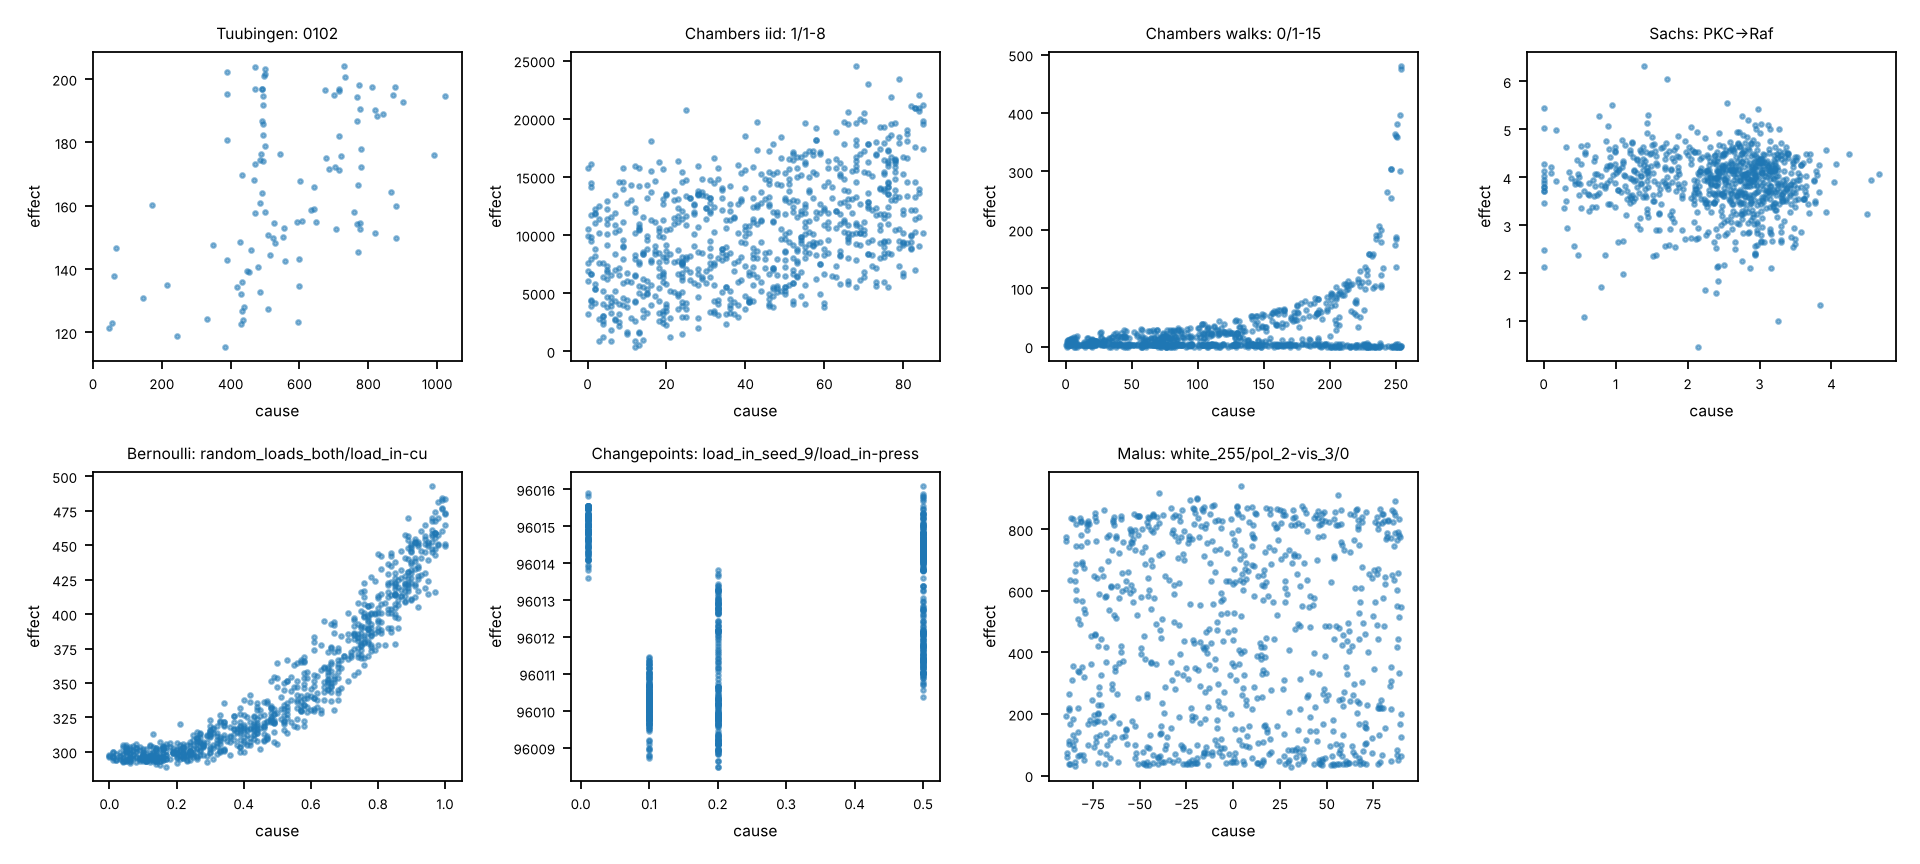
\includegraphics[width=\linewidth]{figs/examples.png}
\caption{One randomly chosen pair (seed $7$) from each collection; $800$ random rows, cause on the horizontal axis.}
\label{fig:examples}
\end{figure}



\begin{table}[t]
\caption{T\"ubingen: mean residual heteroscedasticity $h$ (true direction) on the pairs a rule orients wrongly and rightly; $p$: one-sided Mann--Whitney test that $h$ is larger on the wrong pairs. Twelve rules; $p_{\rm adj}$: Holm over the twelve.}
\label{tab:h2}
\small
\begin{tabular}{@{}lccccc@{}}
\toprule
Rule & wrong/right & $h$ wrong & $h$ right & $p$ & $p_{\rm adj}$\\
\midrule
IGCI & 45/57 & 0.19 & 0.22 & 0.707 & 1\\
RECI & 40/62 & 0.25 & 0.17 & 0.0214 & 0.165\\
ANM-HSIC & 40/62 & 0.32 & 0.13 & 2.67e-09 & 3.2e-08\\
Pairwise LiNGAM & 40/62 & 0.22 & 0.19 & 0.245 & 0.736\\
PDM & 61/41 & 0.22 & 0.18 & 0.0206 & 0.165\\
LOCI & 36/66 & 0.27 & 0.17 & 0.00141 & 0.0141\\
ANM, Gaussian process & 42/53 & 0.29 & 0.10 & 2.83e-09 & 3.2e-08\\
Compression, floor256 & 40/62 & 0.22 & 0.19 & 0.0879 & 0.452\\
Compression, floor256, raw & 36/66 & 0.22 & 0.19 & 0.0946 & 0.452\\
TRA & 29/53 & 0.26 & 0.17 & 0.00405 & 0.0365\\
Compression, round255 & 34/68 & 0.23 & 0.19 & 0.0753 & 0.452\\
AVICI & 42/60 & 0.18 & 0.22 & 0.926 & 1\\
RESIT & 37/60 & 0.34 & 0.13 & 7.98e-10 & 1.04e-08\\
\bottomrule
\end{tabular}
\end{table}

\section{Graph benchmarks}\label{sec:graphs}

The same question for graphs. We score skeletons only, against the 17-arc Sachs consensus (853 cells, log scale) and against the documented graphs of Causal Chambers recordings: two i.i.d.\ recordings (ten random subsamples of $4000$ shuffled rows each), two further recordings with an effective sample size above $1000$, and seventeen new wind-tunnel and light-tunnel recordings whose actuators are random walks and whose effective sample size, by the heuristic $n(1-\rho)/(1+\rho)$, is about three out of $4000$ rows. For the walk recordings the first $4000$ rows in time order are used. Table~\ref{tab:graphs} gives precision/recall/$F_1$ for $22$ method configurations: the classical rules (PC at two levels, GES, DirectLiNGAM, NOTEARS, DAGMA, PCMCI+), nine published packages at library defaults (experiment 45; AVICI, GOLEM, NOTEARS-MLP, GraN-DAG, DAG-GNN, GRaSP, BOSS, RESIT, CAM-UV), BF-BIC with BOSS, and the methods we developed (PC with a nonparametric test, BTAD, LRG, sequential certificates, Appendix~\ref{app:negative}).

\begin{table}[t]
\caption{Skeleton precision/recall/$F_1$ against the reference (strict), mean over data sets. Sachs: one data set; Chambers iid: $2\times10$ subsamples; ESS$>1000$: $2$ recordings; ESS$<20$: $17$ recordings. A number in parentheses is the number of data sets on which the method finished within $900$\,s when fewer than the full number. Experiments 36, 39, 43, 45.}
\label{tab:graphs}
\scriptsize
\setlength{\tabcolsep}{2pt}
\begin{tabular}{@{}lcccc@{}}
\toprule
Method & Sachs & Chambers iid & ESS $>1000$ & ESS $<20$\\
\midrule
PC $\alpha=$0.05 & 1.00/0.41/0.58 & 0.40/0.38/0.37 & 0.48/0.28/0.35 & 0.36/0.39/0.37\\
PC $\alpha=$0.01 & 1.00/0.35/0.52 & 0.39/0.33/0.34 & 0.51/0.27/0.36 & 0.36/0.36/0.36\\
GES-BIC & 1.00/0.41/0.58 & 0.45/0.64/0.49 & 0.74/0.67/0.70 & 0.26/0.71/0.38\\
DirectLiNGAM & 1.00/0.35/0.52 & 0.55/0.60/0.55 & 0.71/0.63/0.66 & 0.26/0.63/0.37\\
NOTEARS & 1.00/0.18/0.30 & 0.41/0.21/0.27 & 0.33/0.24/0.26 & 0.26/0.45/0.33\\
DAGMA & 1.00/0.29/0.45 & 0.44/0.33/0.36 & 0.44/0.41/0.39 & 0.25/0.52/0.34\\
PCMCI+ & 1.00/0.35/0.52 & 0.39/0.33/0.34 & 0.53/0.29/0.37 & 0.27/0.17/0.20\\
GRaSP & 1.00/0.35/0.52 & 0.53/0.57/0.52 & 0.78/0.63/0.68 & 0.27/0.50/0.35\\
BOSS & 1.00/0.35/0.52 & 0.57/0.61/0.55 & 0.77/0.57/0.65 & 0.29/0.54/0.37\\
BF-BIC + BOSS & 0.90/0.53/0.67 & 0.43/0.63/0.49 & 0.57/0.61/0.58 & 0.30/0.68/0.42\\
NOTEARS-MLP & 0.88/0.41/0.56 & 0.42/0.51/0.43 & 0.45/0.27/0.34 (1) & 0.17/0.25/0.21 (1)\\
GOLEM & 1.00/0.18/0.30 & 0.26/0.39/0.31 & 0.36/0.49/0.41 & 0.25/0.47/0.33\\
DAG-GNN & 1.00/0.18/0.30 & 0.36/0.45/0.36 & 0.45/0.34/0.38 & 0.27/0.45/0.34 (16)\\
GraN-DAG & 1.00/0.06/0.11 & 0.55/0.04/0.06 & 0.20/0.04/0.06 & 0.54/0.07/0.12\\
RESIT & 0.39/0.53/0.45 & 0.33/0.80/0.43 & 0.37/0.74/0.49 & 0.23/0.99/0.37\\
CAM-UV & 1.00/0.06/0.11 & 0.67/0.31/0.42 & 0.74/0.43/0.53 & 0.06/0.01/0.02 (15)\\
AVICI & 0.88/0.41/0.56 & 0.48/0.36/0.37 (14) & 0.54/0.17/0.26 & 0.36/0.23/0.28 (8)\\
PC-GCM $\alpha=$0.05 & 0.89/0.47/0.62 & 0.38/0.33/0.34 & 0.54/0.34/0.41 & 0.35/0.54/0.42\\
PC-GCM $\alpha=$0.01 & 1.00/0.47/0.64 & 0.39/0.30/0.32 & 0.47/0.26/0.33 & 0.34/0.46/0.39\\
BTAD & 0.89/0.47/0.62 & 0.56/0.36/0.41 & 0.82/0.46/0.58 & 0.60/0.16/0.25\\
LRG & 0.90/0.53/0.67 & 0.39/0.48/0.43 & 0.52/0.55/0.53 & 0.51/0.28/0.36\\
CERT-CD nonparametric & 1.00/0.29/0.45 & 0.29/0.16/0.20 & 0.60/0.18/0.28 & 0.24/0.87/0.37\\
\bottomrule
\end{tabular}
\end{table}

\paragraph{The ranking depends on the family.} On the i.i.d.\ chamber recordings the best are DirectLiNGAM and BOSS ($F_1=0.55$) and GRaSP ($0.52$); on the two recordings with a large effective sample size GES ($0.70$), GRaSP ($0.68$) and DirectLiNGAM ($0.66$); on Sachs LRG and BF-BIC with BOSS ($0.67$), PC with the nonparametric test ($0.62$--$0.64$) and BTAD ($0.62$), against $0.58$ for PC and GES. No method has a strict $F_1$ above $0.42$ on the seventeen random-walk recordings, where most methods report tens of false edges. The neural methods are weaker: GraN-DAG finds almost no edges ($F_1\le0.12$), GOLEM and DAG-GNN report $22$ to $36$ false edges per recording, NOTEARS with an MLP timed out on $16$ of $17$ walk recordings ($16$ variables) and AVICI on $9$ of $17$ and on $6$ of $20$ i.i.d.\ subsamples; their means in Table~\ref{tab:graphs} are over the data sets on which they finished and are not comparable to the others.

\paragraph{Resolution and structure of the benchmarks.} One Sachs arc changes recall by $0.06$; $16$ of $22$ configurations have a bootstrap interval that contains the best $F_1$ (Section~\ref{sec:noise}). The chamber graphs are bipartite (actuators to sensors), so skeleton recovery is feature selection from actuators to measurements, and the actuators are recognisable by their marginals (Section~\ref{sec:marg}). An interventional pilot on the light tunnel (a pilot, not pre-specified; \texttt{results/lt\_interventions\_check.json}) shows how little a graph benchmark with documented interventions leaves to a new method: a two-sample test of each sensor against the reference recording under each actuator intervention has precision $1.00$ and recall $0.72$ ($28$ of the $39$ arcs among observed variables, which here are also the ancestral pairs; AUC $0.91$ from the $p$-values), and the missed arcs, all from light sources to their sensors, show no shift in the data ($p$ between $0.06$ and $0.86$); a conditional version (residuals of a boosted regression on the estimated non-descendants) raises recall to $0.79$ at a precision of $0.51$.

\paragraph{What we do not conclude.} The reference networks are small, the Sachs consensus is contested, and several baselines (CAM, SCORE) were not run. The differences between graph methods are mostly within sampling error, and the effective sample size of the walk recordings limits what any method can show. We read the graph results as consistent with the pair results: no rule leads across families.



\section{Selective subsets}\label{app:subsets}


Pair benchmarks are often evaluated on a subset of pairs (a given variable type or sample size, or pairs where the other rules disagree). We drew $10000$ random subsets of $50$ of the $102$ pairs. The accuracy of a rule on a subset has a standard deviation of about $0.05$. For the eight rules whose full-sample accuracy is within $0.04$ of RECI the probability that a rule beats RECI on a subset lies between $0.34$ and $0.71$, so most subsets would support either order; for round255 compression, $0.059$ above RECI, it is $0.79$. The expected best accuracy over $m$ independently drawn subsets, which is what a researcher reports after trying $m$ subsets and keeping the best, grows with $m$: RECI $0.608$ ($m=1$), $0.650$ ($3$), $0.684$ ($10$); LOCI $0.647$, $0.688$, $0.722$; round255 compression $0.667$, $0.707$, $0.740$. The inflation at $m=10$ is seven to eight points for every rule, which leaves the order of the rules unchanged; what it changes is the claim of an absolute level. Each subset is half of the same $102$ pairs, so this measures selection noise about a known full-sample accuracy, not how a researcher actually chooses subsets (by type or size, not at random).







\section{Tables moved from the main text}
\begin{table}[ht]
\caption{Accuracy (fraction of pairs oriented correctly; exact ties half) of twelve rules on eight collections. All rules see the raw arrays, except that T\"ubingen is dequantised (Section~\ref{sec:rules}). ``--'': not run, or no value for most pairs (TRA on the changepoint collection; PDM and the first compression implementation only on the original collections). ``Walks (19)'' contains all $19$ untouched recordings ($486$ pairs; the $122$ pairs of ``walks'' come from five of them). The new collections have $8$, $7$ and $4$ distinct edges; intervals that account for clusters are in Appendix Table~\ref{tab:collections_ci}.}
\label{tab:collections2}
\small
\setlength{\tabcolsep}{3.2pt}
\begin{tabular}{@{}lcccccccc@{}}
\toprule
Rule & T\"ub. & iid & walks & Walks & Sachs & Bern. & Chgpt. & Malus\\
 & (102) & (94) & (122) & (19: 486) & (17) & (16) & (70) & (48)\\
\midrule
IGCI & 0.56 & 0.94 & 0.89 & 0.96 & 0.65 & 1.00 & 1.00 & 0.08\\
RECI & 0.61 & 0.98 & 0.94 & 0.83 & 0.53 & 0.25 & 1.00 & 0.56\\
ANM-HSIC & 0.61 & 0.72 & 0.63 & 0.43 & 0.59 & 0.31 & 0.57 & 0.31\\
Pairwise LiNGAM & 0.61 & 0.78 & 0.71 & 0.67 & 0.53 & 0.88 & 0.43 & 0.40\\
PDM & 0.40 & 0.93 & 0.84 & -- & -- & -- & -- & --\\
LOCI & 0.65 & 0.77 & 0.68 & -- & 0.47 & 0.56 & 0.80 & 0.38\\
ANM, Gaussian process & 0.55 & 0.77 & 0.67 & -- & 0.56 & 0.47 & 0.54 & 0.33\\
Compression, floor256 & 0.61 & 0.30 & 0.61 & -- & 0.76 & -- & -- & --\\
Compression, round255 & 0.67 & 0.38 & 0.52 & 0.50 & 0.65 & 0.50 & 1.00 & 0.60\\
TRA & 0.65 & 0.86 & 0.61 & 0.56 & 0.59 & 0.62 & -- & 0.54\\
AVICI & 0.59 & 0.90 & 0.56 & 0.63 & 0.53 & 0.62 & 0.40 & 0.02\\
RESIT & 0.61 & 0.71 & 0.65 & 0.48 & 0.47 & 0.25 & 0.53 & 0.50\\
\bottomrule
\end{tabular}
\end{table}

\begin{table}[ht]
\caption{Rules on the 102 T\"ubingen pairs: unweighted accuracy with a 95\% interval (TRA: the $82$ pairs on which it returned a value) and the multiverse summary of Section~\ref{sec:multi}. ``Range'': minimum and maximum accuracy over the ten reporting universes with at least $30$ pairs per rule; ``Rank'': best and worst rank; ``First'': universes in which the rule is first (ties share the rank); ``$>$RECI'': universes in which it is above RECI; ``Best of 10'': expected best accuracy after trying ten random subsets of $50$ pairs.}
\label{tab:multi}
\small
\setlength{\tabcolsep}{3pt}
\begin{tabular}{@{}lcccccc@{}}
\toprule
Rule & Accuracy [interval] & Range & Rank & First & $>$RECI & Best of 10\\
\midrule
IGCI & 0.559 [0.46, 0.66] & 0.47--0.71 & 4--12 & 0 & 0 & 0.635\\
RECI & 0.608 [0.51, 0.70] & 0.61--0.87 & 1--6 & 1 & 0 & 0.684\\
ANM-HSIC & 0.608 [0.51, 0.70] & 0.57--0.70 & 3--12 & 0 & 1 & 0.682\\
Pairwise LiNGAM & 0.608 [0.51, 0.70] & 0.54--0.74 & 4--13 & 0 & 0 & 0.682\\
PDM & 0.402 [0.31, 0.50] & 0.40--0.61 & 10--13 & 0 & 0 & 0.477\\
LOCI & 0.647 [0.55, 0.74] & 0.63--0.77 & 1--9 & 1 & 2 & 0.722\\
ANM, Gaussian process & 0.554 [0.45, 0.65] & 0.55--0.75 & 3--12 & 0 & 0 & 0.628\\
Compression, floor256 & 0.608 [0.51, 0.70] & 0.61--0.79 & 3--8 & 0 & 0 & 0.686\\
Compression, floor256, raw rows & 0.647 [0.55, 0.74] & 0.64--0.76 & 2--8 & 0 & 2 & 0.721\\
TRA & 0.646 [0.53, 0.75] & 0.65--0.76 & 2--6 & 0 & 4 & 0.729\\
Compression, round255 & 0.667 [0.57, 0.76] & 0.67--0.88 & 1--3 & 8 & 9 & 0.740\\
AVICI & 0.588 [0.49, 0.68] & 0.54--0.65 & 5--12 & 0 & 0 & 0.665\\
RESIT & 0.613 [0.52, 0.71] & 0.47--0.66 & 5--13 & 0 & 1 & 0.686\\
\bottomrule
\end{tabular}
\end{table}

\begin{table}[ht]
\caption{T\"ubingen, $50$ protocol configurations (five row caps $\times$ dequantisation or not $\times$ five seeds). Range of the unweighted and of the official-weight accuracy over all configurations, and the range (in points) between the best and the worst level of each factor, averaged over the others.}
\label{tab:protocol}
\small
\begin{tabular}{@{}lccccc@{}}
\toprule
Rule & unweighted & weighted & rows & dequant. & seed\\
\midrule
IGCI (ours, uniform ref.) & 0.49--0.66 & 0.57--0.68 & 1 & 11 & 1\\
RECI & 0.56--0.67 & 0.58--0.73 & 2 & 1 & 2\\
ANM-HSIC & 0.54--0.61 & 0.52--0.60 & 3 & 0 & 2\\
Pairwise LiNGAM & 0.56--0.64 & 0.58--0.67 & 2 & 0 & 3\\
Compression, round255 & 0.61--0.71 & 0.60--0.78 & 2 & 1 & 1\\
IGCI (cdt, Gaussian ref.) & 0.40--0.63 & 0.40--0.64 & 1 & 18 & 0\\
RECI (cdt) & 0.60--0.68 & 0.66--0.79 & 2 & 2 & 1\\
CDS (cdt) & 0.54--0.66 & 0.50--0.65 & 7 & 4 & 2\\
\bottomrule
\end{tabular}
\end{table}

\begin{table}[ht]
\caption{Accuracy of rules under two tie conditions (raw arrays; $10^{-6}$ range jitter on tied values), same pairs (experiment 59). T\"ubingen is dequantised in both. cdt: \texttt{cdt} package defaults.}
\label{tab:ties}
\small
\setlength{\tabcolsep}{3pt}
\begin{tabular}{@{}llccccccc@{}}
\toprule
Rule & Ties & T\"ub. & iid & walks & Sachs & Bern. & Chgpt. & Malus\\
\midrule
IGCI (ours, uniform reference) & raw & 0.56 & 0.94 & 0.89 & 0.65 & 1.00 & 1.00 & 0.08\\
IGCI (ours, uniform reference) & jitter & 0.56 & 0.06 & 0.13 & 0.47 & 0.00 & 0.00 & 0.94\\
IGCI (cdt, Gaussian reference) & raw & 0.42 & 0.94 & 0.84 & 0.47 & 1.00 & 1.00 & 0.08\\
IGCI (cdt, Gaussian reference) & jitter & 0.42 & 0.06 & 0.12 & 0.53 & 0.00 & 0.00 & 0.94\\
ANM-HSIC & raw & 0.57 & 0.73 & 0.62 & 0.59 & 0.31 & 0.57 & 0.31\\
ANM-HSIC & jitter & 0.57 & 0.72 & 0.62 & 0.59 & 0.31 & 0.47 & 0.33\\
RECI & raw & 0.61 & 0.98 & 0.94 & 0.53 & 0.25 & 1.00 & 0.56\\
RECI & jitter & 0.61 & 0.98 & 0.94 & 0.53 & 0.25 & 1.00 & 0.56\\
Pairwise LiNGAM & raw & 0.61 & 0.78 & 0.71 & 0.53 & 0.88 & 0.43 & 0.40\\
Pairwise LiNGAM & jitter & 0.61 & 0.78 & 0.71 & 0.53 & 0.88 & 0.43 & 0.40\\
\bottomrule
\end{tabular}
\end{table}

\begin{table}[ht]
\caption{Reproduction of the compression baseline on the $102$ T\"ubingen pairs (official weights). The published value is $68$ of $102$ pairs, $74.7\%$ weighted.}
\label{tab:audit}
\small
\begin{tabular}{@{}lccc@{}}
\toprule
Quantisation and rows & pairs correct & unweighted & weighted\\
\midrule
$\lfloor 256q\rfloor$, all rows & 67 & 0.657 & 0.688\\
$\lfloor 255q\rfloor$, all rows & 71 & 0.696 & 0.705\\
$\mathrm{round}(255q)$, all rows & 68 & 0.667 & 0.747\\
$\mathrm{round}(255q)$, $2000$ rows & 69 & 0.676 & 0.744\\
$\mathrm{round}(255q)$, no thinning & 69 & 0.676 & 0.753\\
$\mathrm{round}(255q)$, $500$ rows & 71 & 0.696 & 0.717\\
floor256, $2000$ random dequantised rows (experiment 42) & 62 & 0.608 & 0.680\\
\bottomrule
\end{tabular}
\end{table}

\begin{table}[ht]
\caption{T\"ubingen accuracy by tercile of $h$ ($34$ pairs per tercile; TRA $24$, $31$, $27$).}
\label{tab:strata}
\small
\begin{tabular}{@{}lccc@{}}
\toprule
Rule & low $h$ & middle & high $h$\\
\midrule
ANM-HSIC & 0.97 & 0.56 & 0.29\\
RESIT & 0.96 & 0.65 & 0.24\\
ANM, Gaussian process & 0.91 & 0.53 & 0.22\\
TRA & 0.83 & 0.68 & 0.44\\
LOCI & 0.82 & 0.62 & 0.50\\
RECI & 0.68 & 0.68 & 0.47\\
IGCI & 0.59 & 0.44 & 0.65\\
Pairwise LiNGAM & 0.65 & 0.53 & 0.65\\
Compression, round255 & 0.74 & 0.74 & 0.53\\
Compression, floor256, raw & 0.71 & 0.68 & 0.56\\
AVICI & 0.53 & 0.56 & 0.68\\
PDM & 0.56 & 0.35 & 0.29\\
\bottomrule
\end{tabular}
\end{table}

\begin{table}[ht]
\caption{Matched simulated pairs: accuracy against the strength $a$ ($100$ pairs per level). Left: noise scale depends on the cause. Right: independent random scale with the same kind of marginal (control).}
\label{tab:dose}
\small
\begin{tabular}{@{}lcccc|cccc@{}}
\toprule
 & \multicolumn{4}{c|}{scale depends on cause} & \multicolumn{4}{c}{independent scale}\\
Rule & $0$ & $0.5$ & $1$ & $1.5$ & $0$ & $0.5$ & $1$ & $1.5$\\
\midrule
ANM-HSIC & 1.00 & 0.49 & 0.12 & 0.21 & 1.00 & 1.00 & 0.99 & 0.89\\
IGCI & 0.64 & 0.72 & 0.91 & 0.99 & 0.64 & 0.73 & 0.95 & 0.99\\
RECI & 0.78 & 0.77 & 0.87 & 0.93 & 0.78 & 0.84 & 0.96 & 0.98\\
\bottomrule
\end{tabular}
\end{table}
